
%%%%%%%%%%%%%%%%%%%%%%%%%%%%%%%%%%%%%%%%%%%%%%%%%%%%%%%%%%%%%%
%\section{Basic Research Questions and Their Evaluations}
\label{sec:hypotheses}

In the previous chapter (\chapt{chap:Contribution}) we proposed an end-user robot programming framework that allows users to teach robots new actions by demonstration, that can be reused with automated planners to complete previously unseen tasks.
We believe that non-robotics expert users without experience in automated planning can easily learn to use this framework.
Thus, %to evaluate the framework's usability for non-expert users, 
%we formulated the following hypotheses
%\begin{enumerate}
%\item[\textbf{H1}] \textit{The user understands the symbolic planning concepts.} This allows us to verify, if the symbolic planning language (PDDL), to describe the world state in terms of object types, properties, generalised properties, and action models, in terms of preconditions and effects, can be adopted easily by non-expert users.
%\item[\textbf{H2}] \textit{The user is able to teach the robot an action model using the proposed framework.} This allows us to evaluate how users operate the framework.
%\end{enumerate} 
we conducted two qualitative user experiments to respond to the following questions:
\begin{enumerate}
  \item[\textbf{Q1}] How do non-expert users adopt the automated planning language with its action model representation? (Section \ref{sec:Exp1})
  \item[\textbf{Q2}] Can users teach a robot action models for automated planning using the robot programming framework? (Section \ref{sec:Exp2})
\end{enumerate}

The experimental context was designed around a Baxter robot (\fig{fig:Baxter}).
In both experiments we included elements to assess the user's understanding of action models used by automated planners.
Understanding this symbolic representation is a key requirement to use the proposed framework.
In the following sections we briefly outline the experimental setup, measurements and results for each experiment.
 
% \begin{table}[t]
% \caption{Description of the world state in PDDL}
% \label{pddl_deschription}
% \begin{center}
% \begin{tabular}{l|l|l|l} \hline
%  \textbf{object name} & \textbf{type} & \textbf{property} & \textbf{generalised property} \\ \hline 
% redCube & cube & (at cube A) & (at ?cube ?posA)\\ \hline 
% A & position & (empty A) & (empty ?posA)\\ \hline 
% \end{tabular}\label{tab:pddl_deschription}
% \end{center}
% \end{table}

% Taken from Paper2 Basic research questions + experiments 1

\section{Experiment 1: Acceptance of Automated Planning and PDDL Concepts}\label{sec:Exp1}

% \section{How do non-expert users adopt the automated planning language with its action model representation?}
%%%%%%%% 1.25 pages %%%%%%%
In this experiment, we are addressing the following question:

\begin{enumerate}
	\item[\textbf{Q1}] How do non-expert users adopt the automated planning language with its action model representation?
\end{enumerate}

Users were introduced to a symbolic planning language (a simplified version of PDDL), involving the STRIPS formalism (\cite{fikes1971strips}) with type structures used in automated planning (\chapt{chap:Sota-AP}).
Users were instructed to describe world state configurations to the robot.
The goal was to assess the user's adoption of the planning concepts (object types, properties, generalised properties, action models) and to verify that the symbolic planning language is appropriate for non-expert users.

\begin{figure}[htp]
	\centering
	\begin{subfigure}[t]{0.24\textwidth}%
		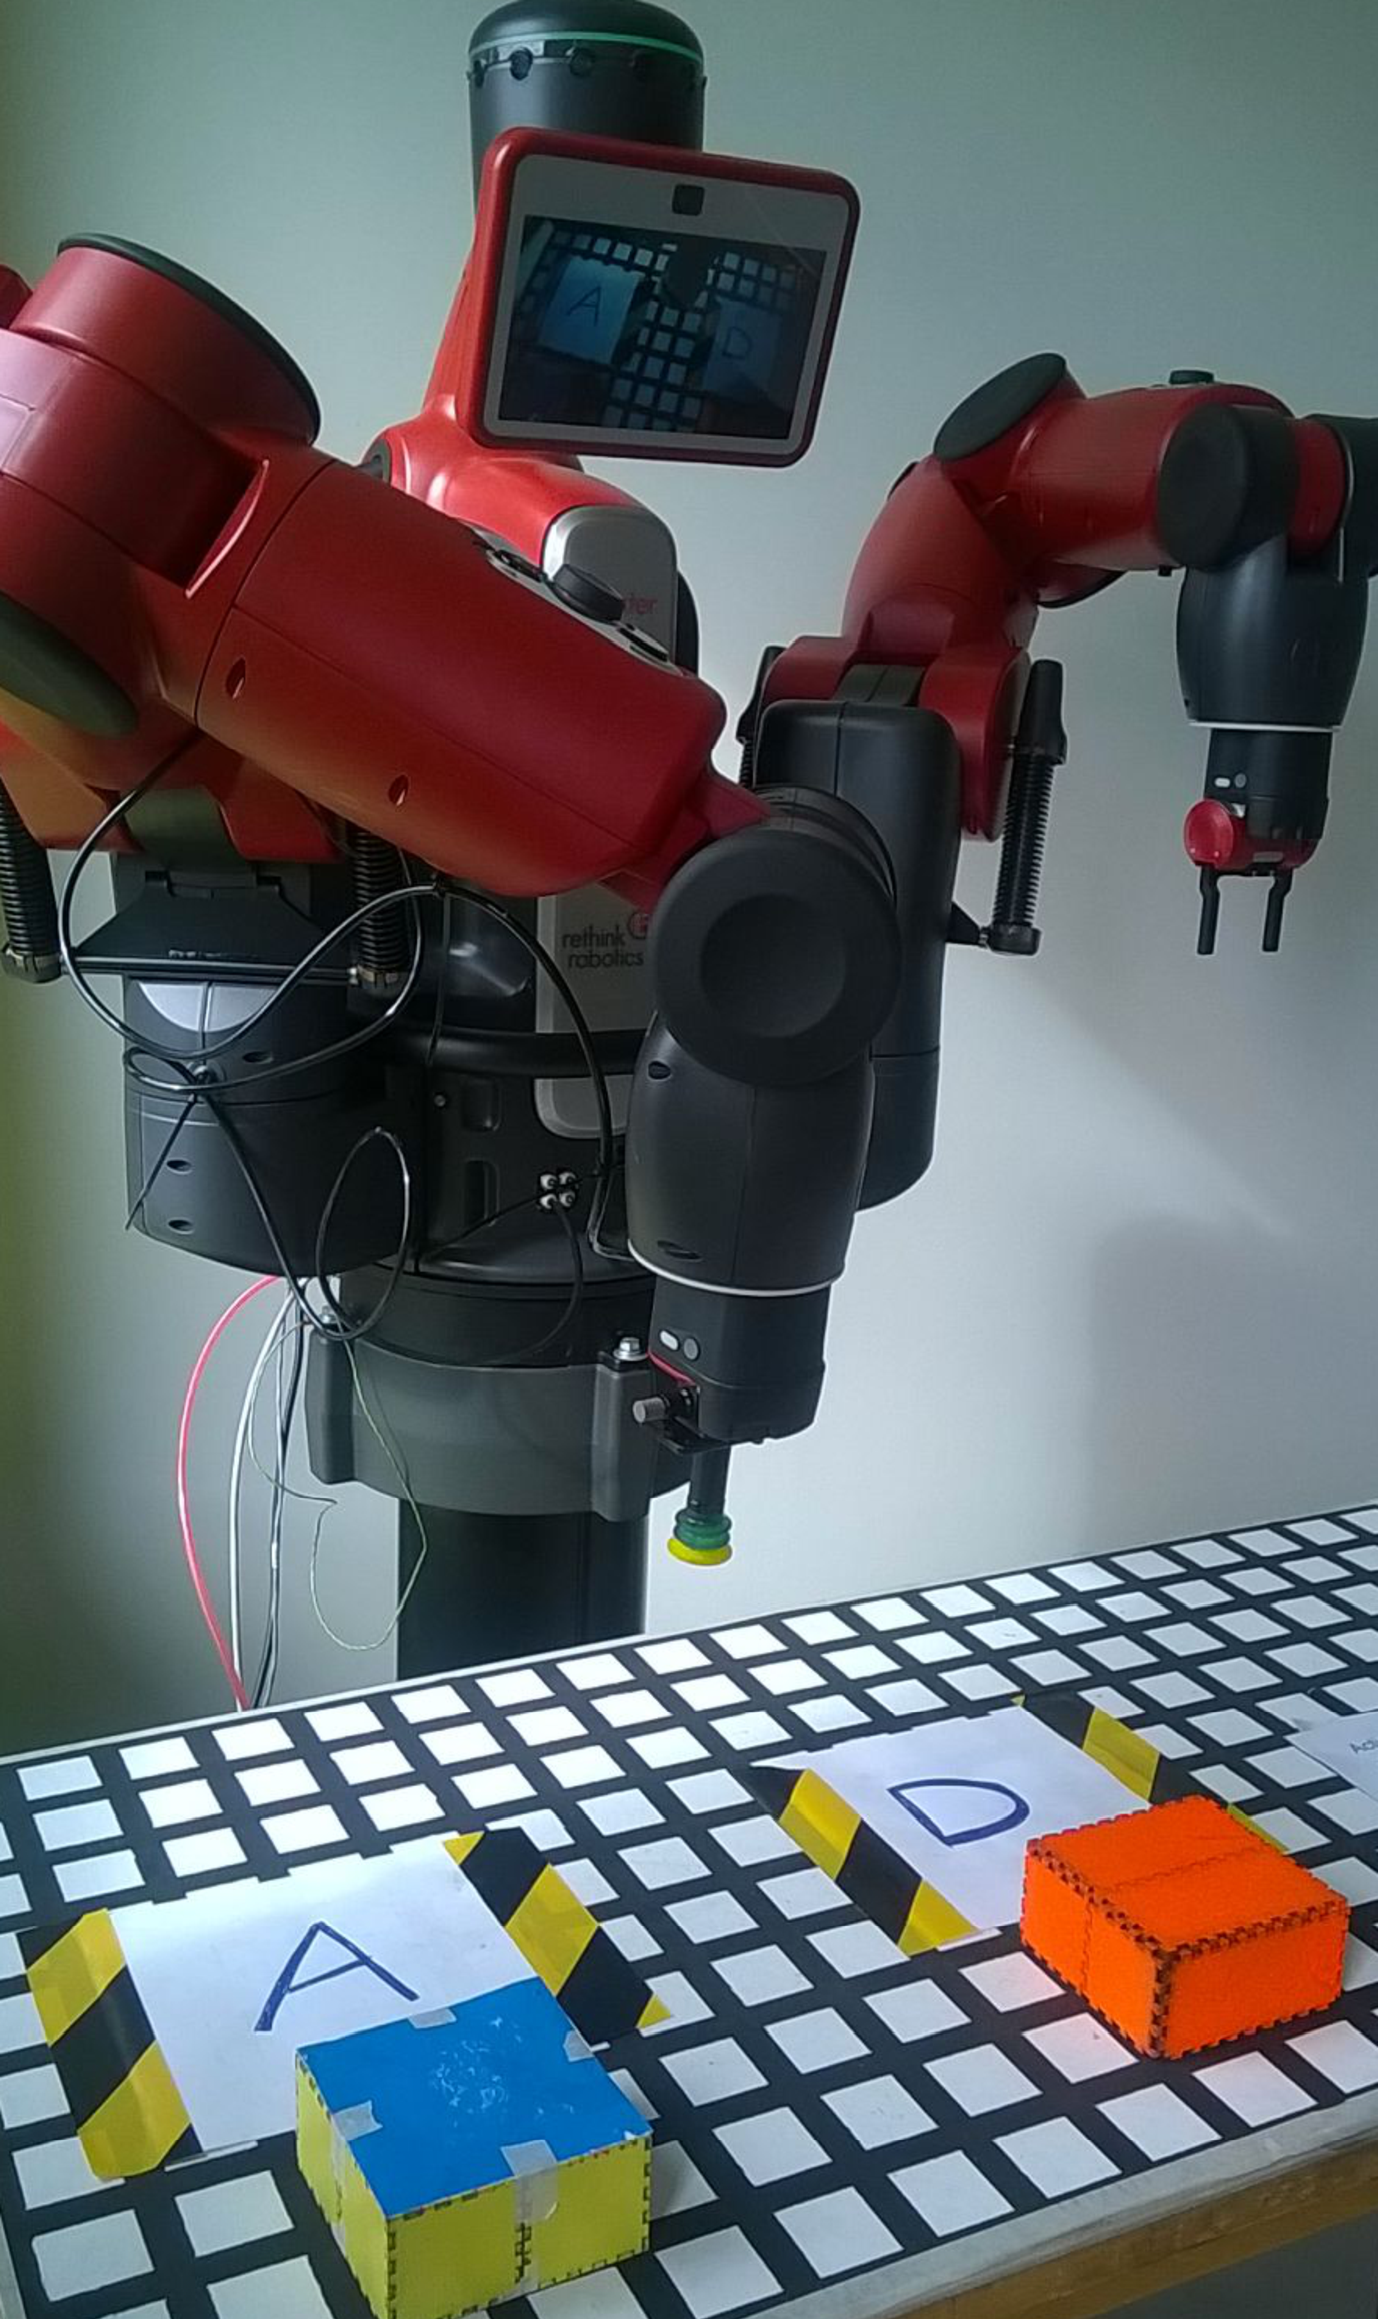
\includegraphics[width=\textwidth]{figures/experiment1}%
		\caption{Baxter robot}\label{fig:Baxter}%
	\end{subfigure}~~%
	\begin{subfigure}[t]{0.24\textwidth}%
		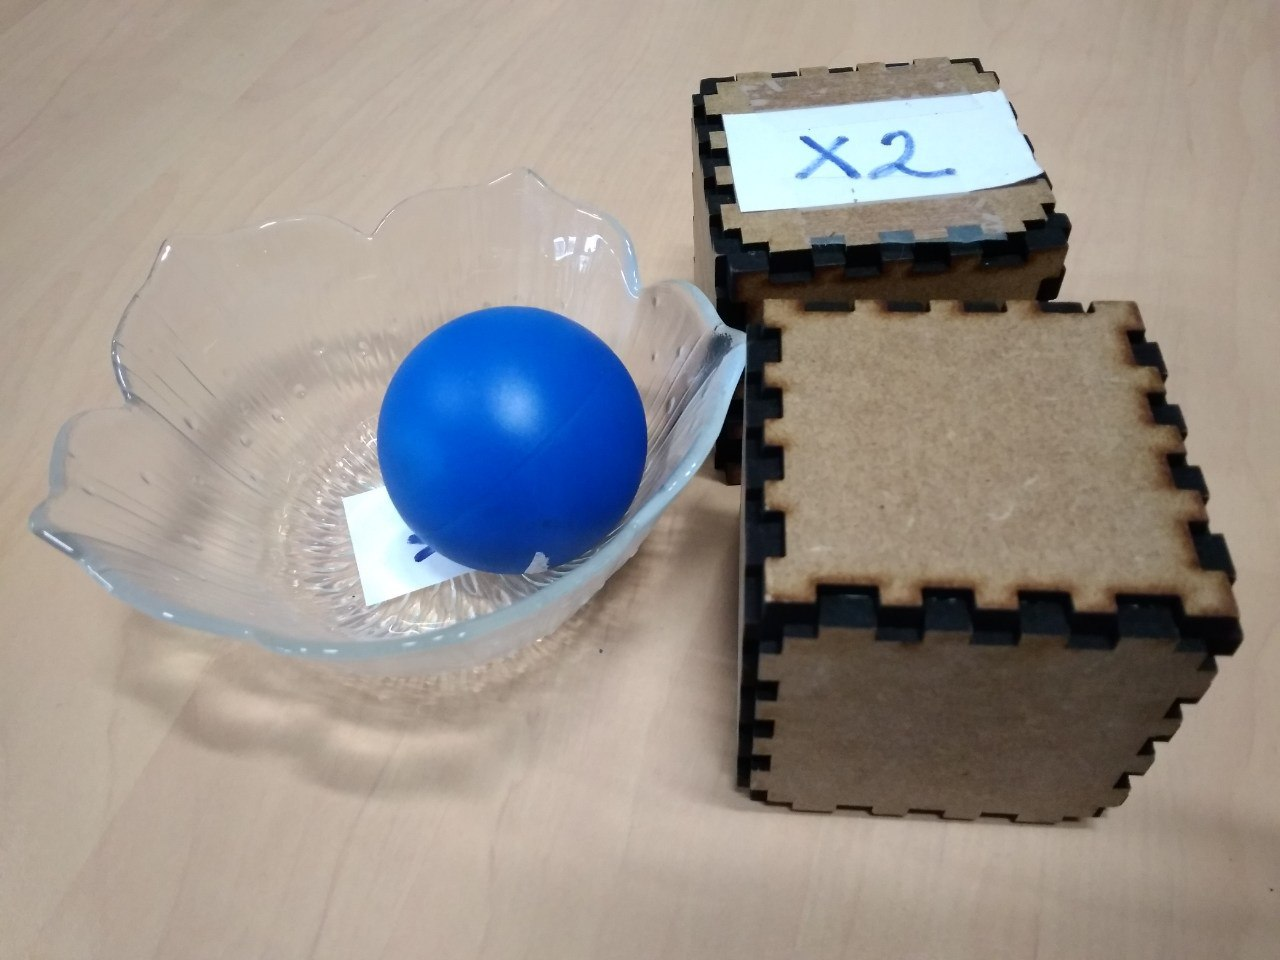
\includegraphics[width=\textwidth]{figures/exp1-setup}%
		\caption{Experiment 1 setup}\label{fig:exp1-setup}%  
	\end{subfigure} 	  
	\caption{Experimental setup for user studies.}
	\label{fig:pre-experiment}%
	% 	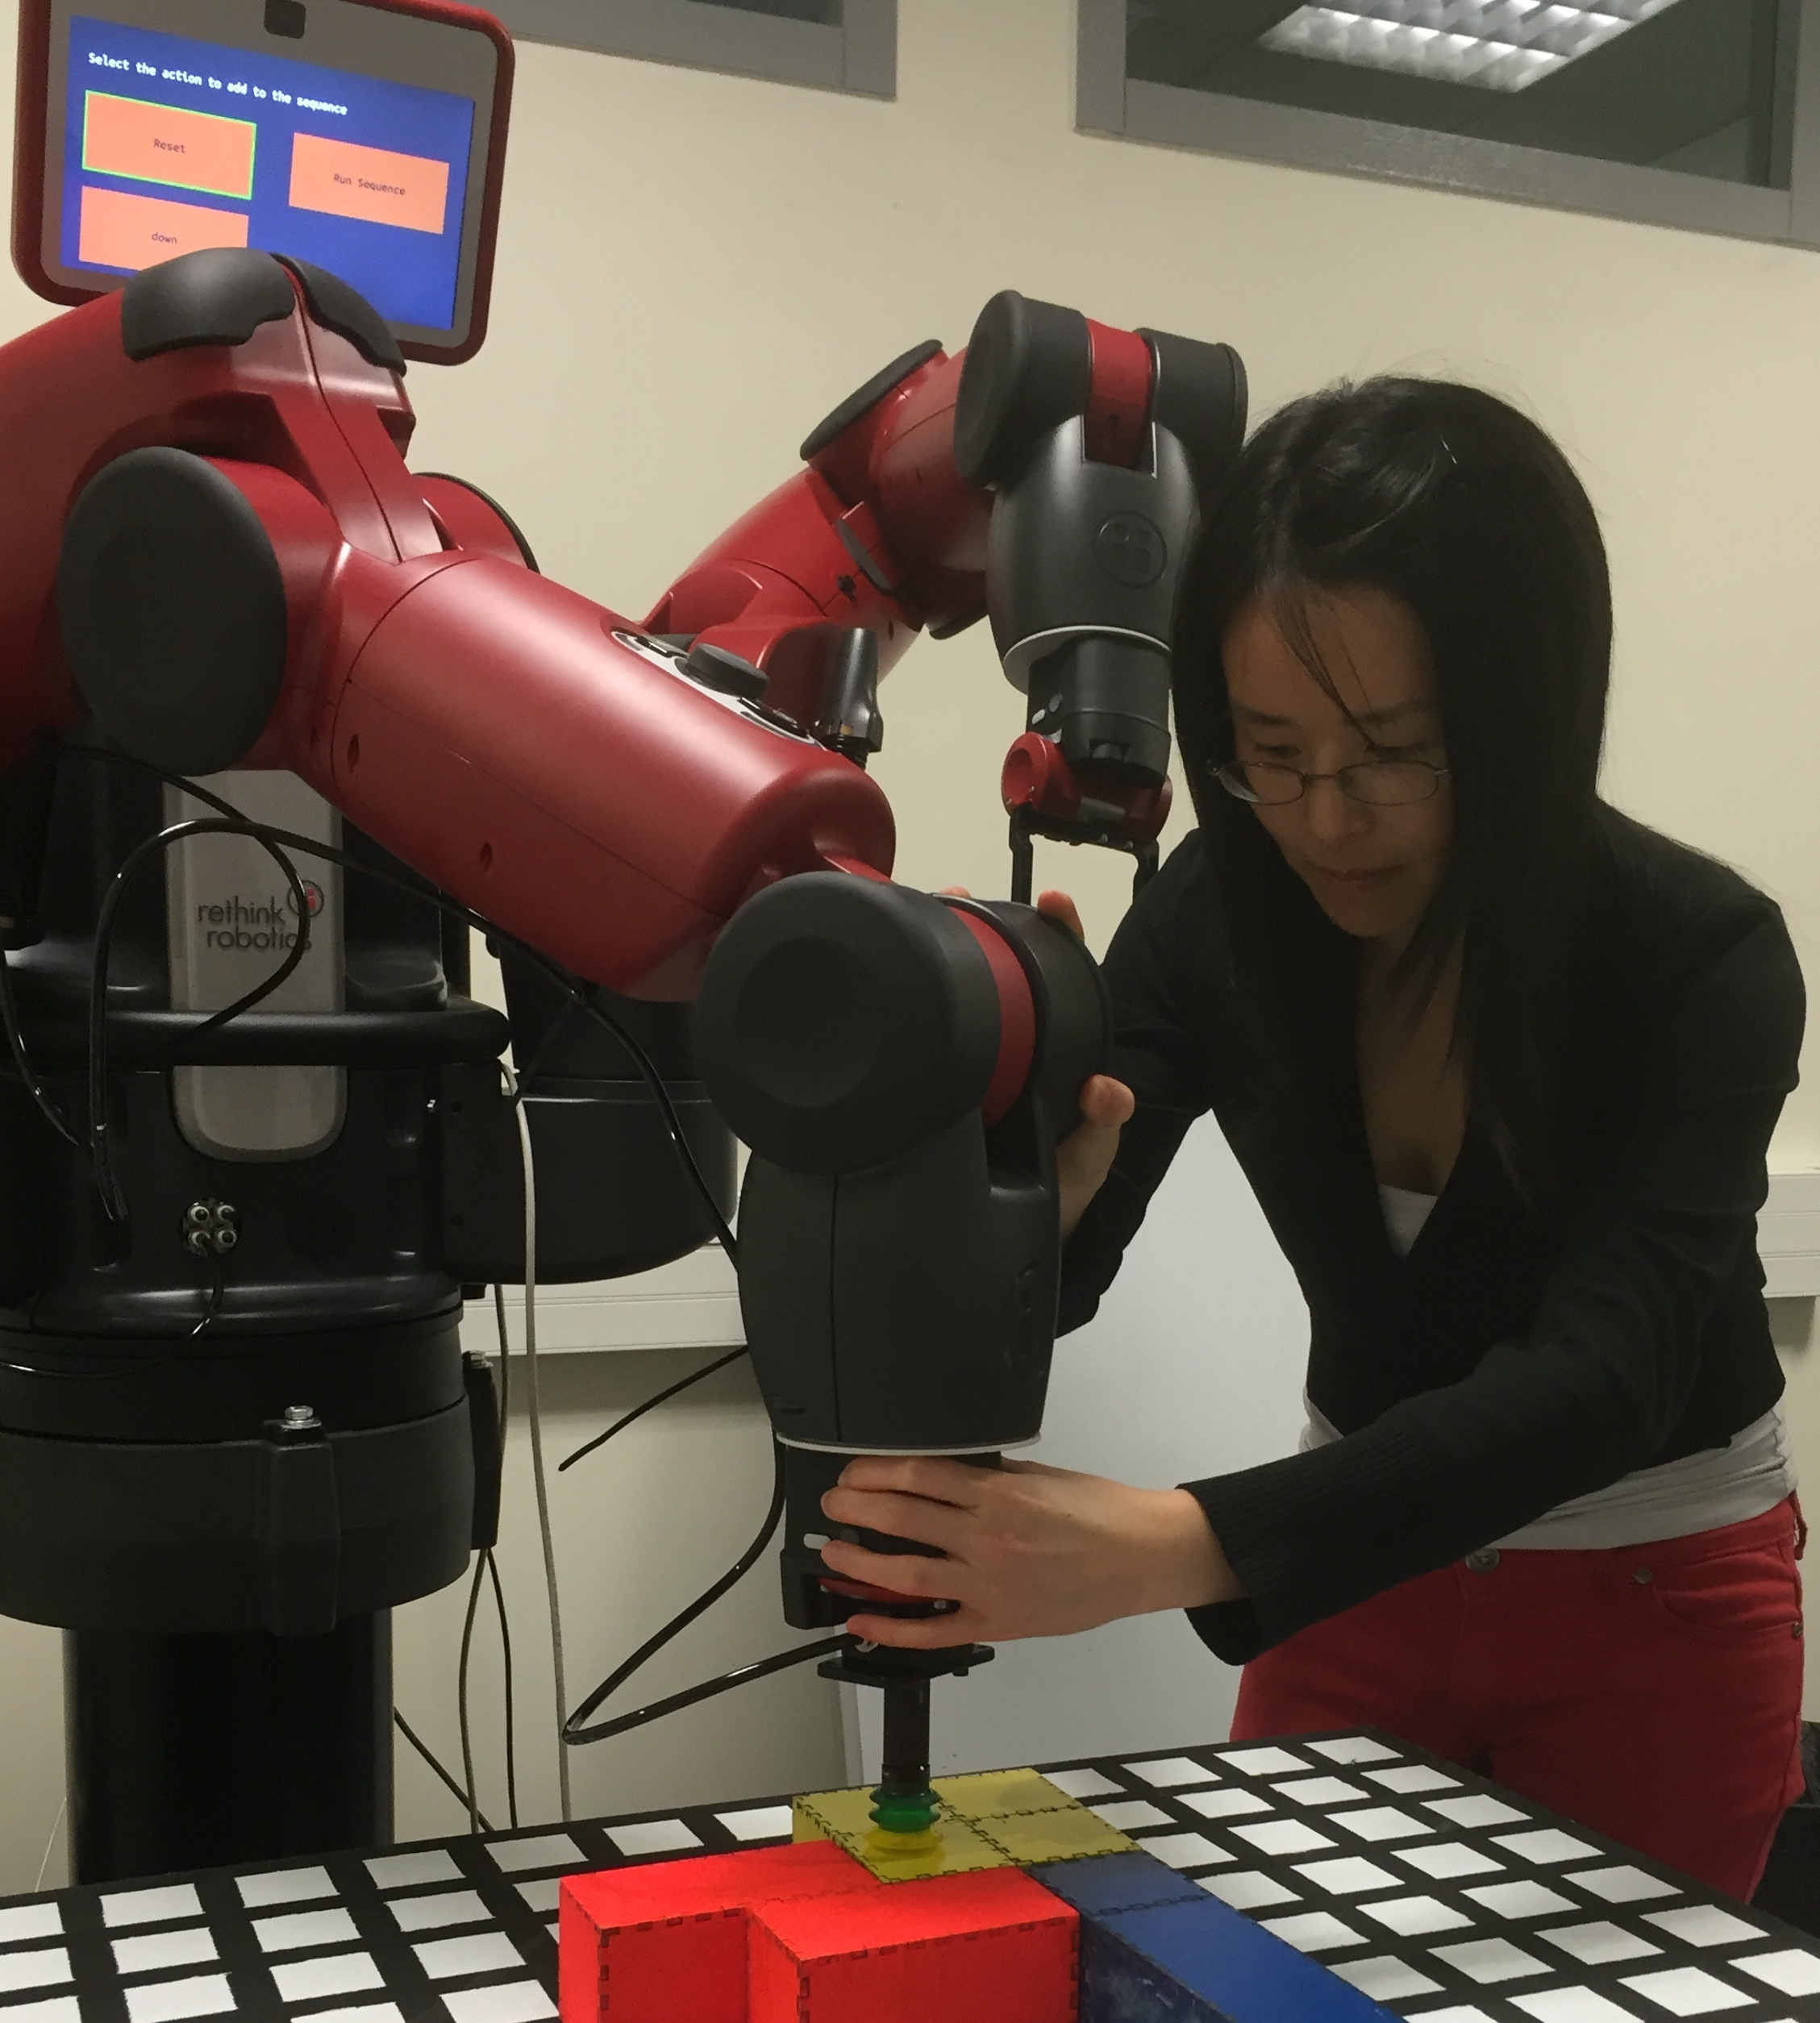
\includegraphics[width=.3\textwidth]{figures/experiment-setup2}
\end{figure}
\subsection{Experimental Setup \& Participants}
We recruited 10 participants (1 male, 9 female), who were sociology students at the Universit\'{e} Grenoble Alpes.
3 participants reported no programming experience, 6  had experience with office productivity software (`beginner'), and 1 had previously taken a programming course before (`advanced').

The experimental setup consisted of a 2x2 board (with positions A1, A2, B1, B2), 2 cubes, 1 ball, and 1 ball recipient in the form of a bowl (\fig{fig:exp1-setup}).
%The experimenter showed the participants a video of the Baxter robot \cite{Baxter}
The participants were given sheets with empty tables to complete for each task.
Each participant was allocated 1 hour, but the average duration of the experiment was 49 minutes.
At the end, participants were given a questionnaire related to their experience and their understanding of the learned planning language and concepts.
The participants' behaviour was observed by the experimenter and the experiment was recorded on camera.
The experimental protocol, questionnaire and additional material used can be found in Appendix \ref{app:exp1}.


%\begin{figure}[h]
%	\centering
%	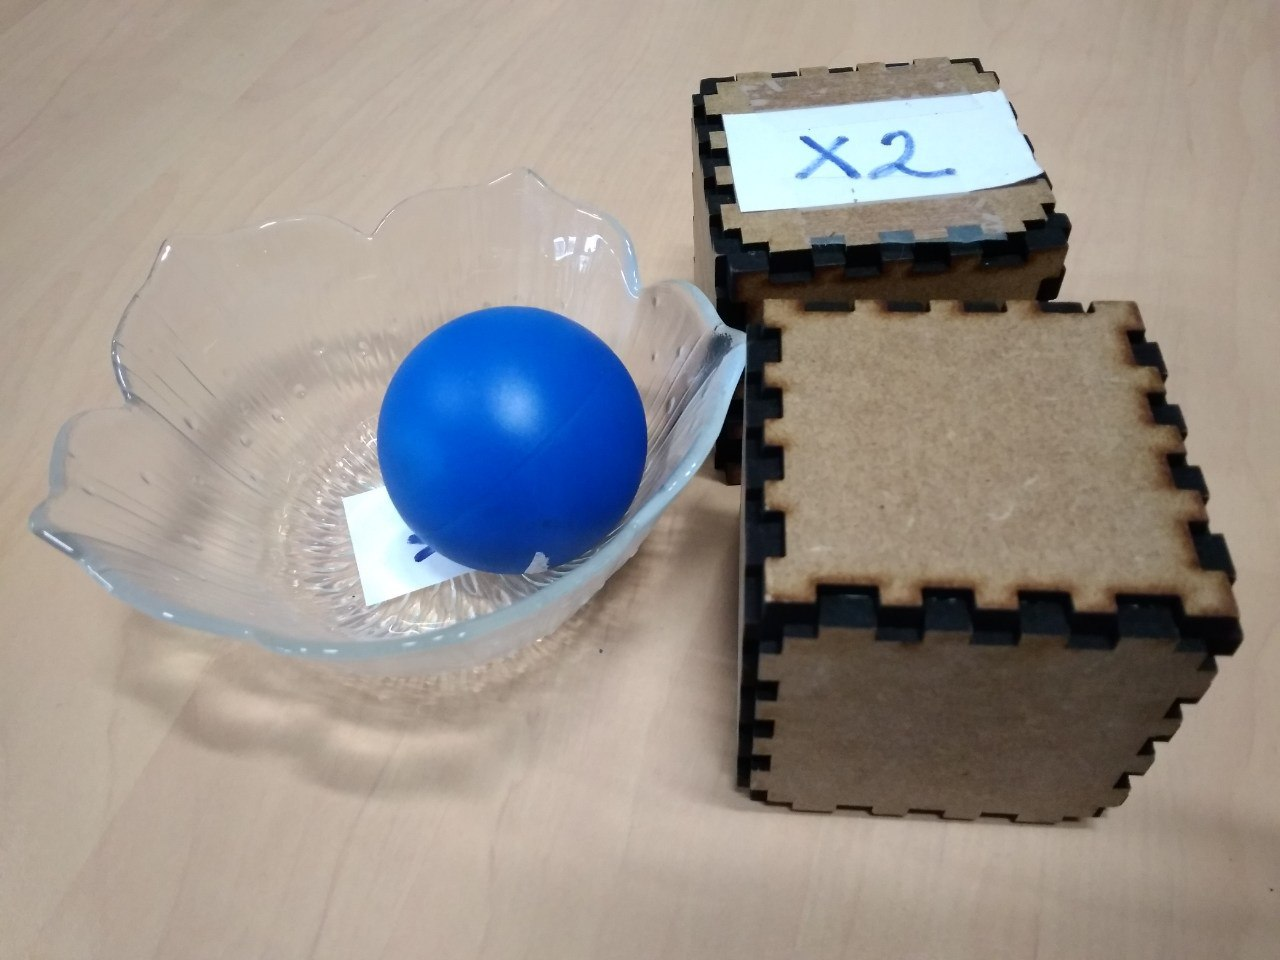
\includegraphics[width=0.65\linewidth]{figures/exp1-setup}
%	\caption{Experiment 1 setup consisted of a 2x2 board, 2 cubes, 1 ball, and 1 ball recipient}
%	\label{fig:exp1-setup}
%\end{figure}
 

\subsection{Experimental Design \& Measurements}
%After a short introduction to the Baxter robot, 
Users were told that they needed to use a symbolic planning language to describe the state of the world and the semantic meaning of actions to the robot. 
Throughout the experiment, users were faced with three different scenarios. 
\fig{fig:scenarios-exp1} shows an example of the experimental design, where the robot's action was to move the ball to an occupied position (B2). 
We evaluated their capability to apply the planning language to different situations.

\begin{figure}[h]
	\centering
	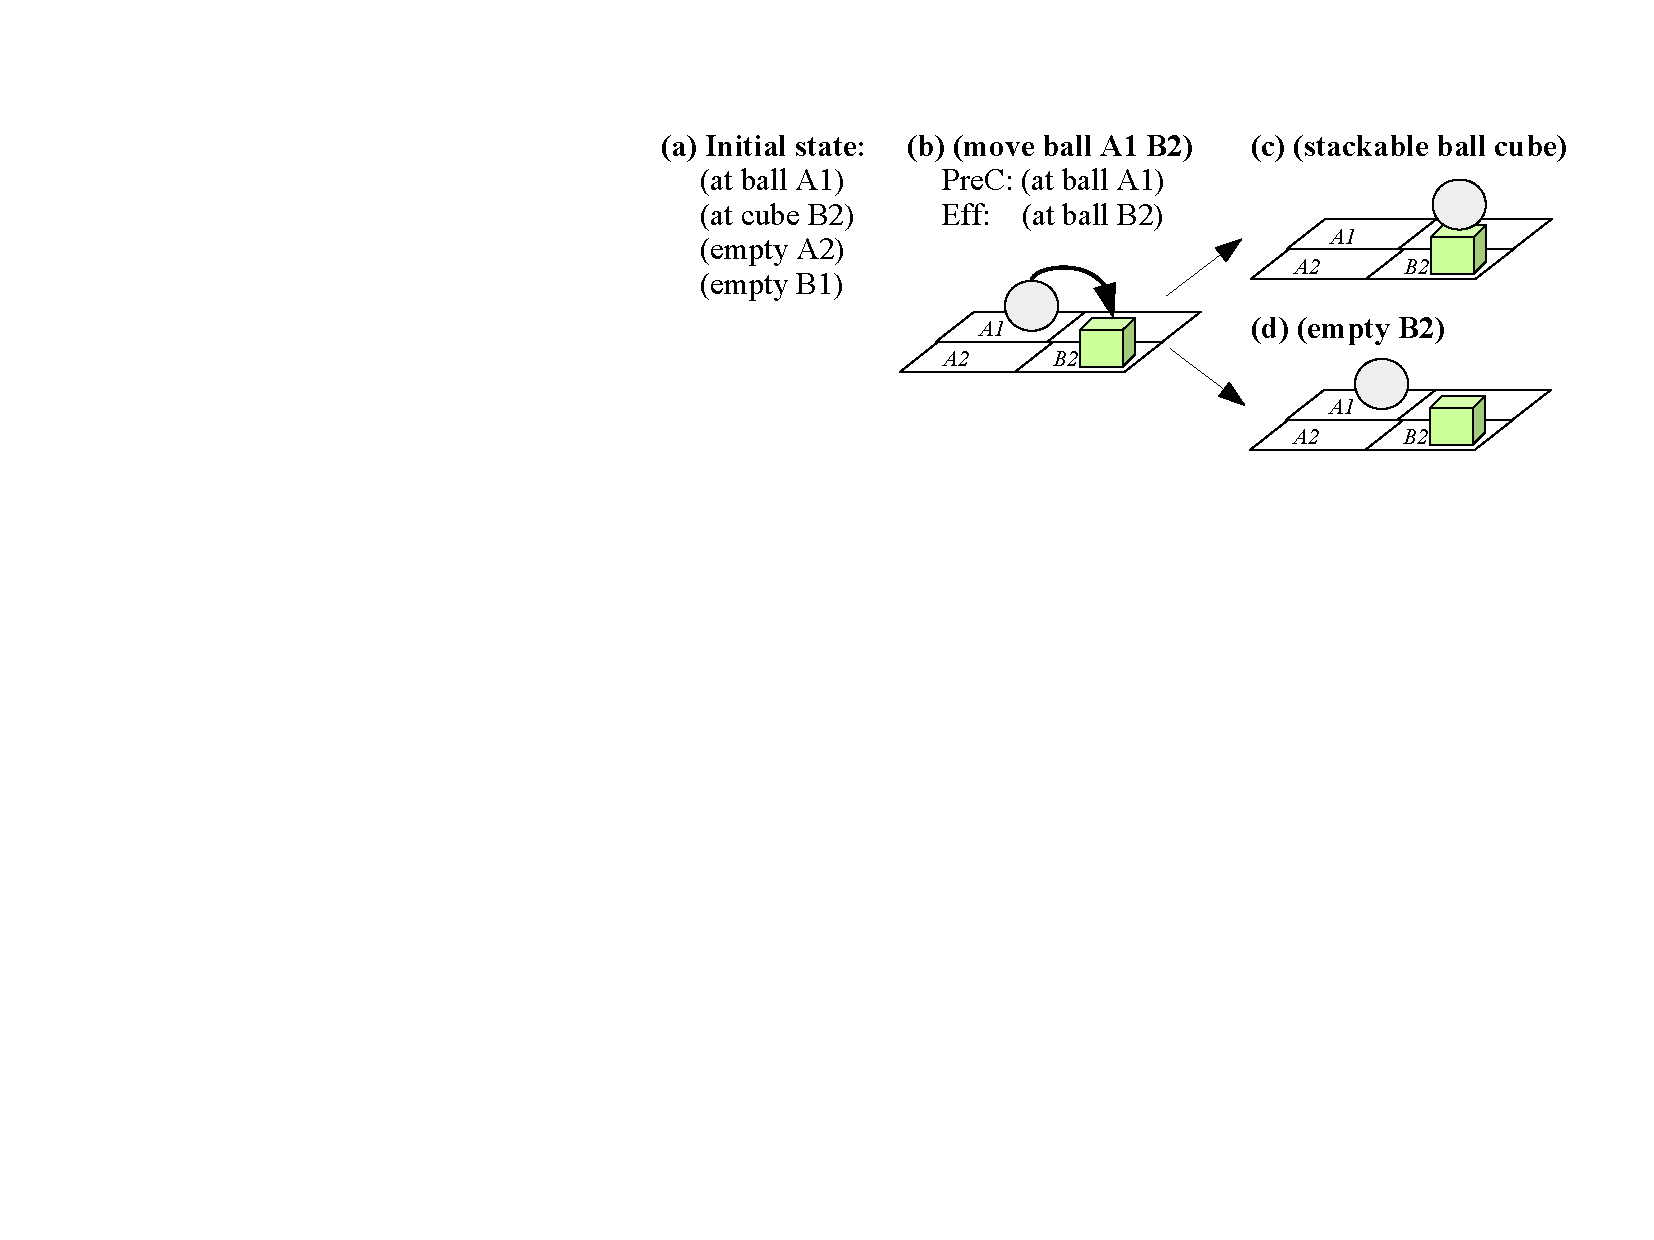
\includegraphics[width=0.75\linewidth]{figures/scenarios-exp1}
	\caption{Users were instructed to provide a description of (a) the initial state of the world and (b) an initial move action model.
		Then they derived additional preconditions for moving the ball from position A1 to B2: (c) \textit{(stackable ball cube)}: the ball can be stacked onto the cube, and (d) \textit{(empty B2)}: if the ball cannot be stacked, the target position should be empty.}
	\label{fig:scenarios-exp1}
\end{figure}

The experiment consisted of the following phases:
\begin{itemize}
%  \item{Introduction: After a short introduction to the Baxter robot \cite{Baxter}, users were told that they needed to use a planning language (STRIPS) to explain Baxter the state of the world and the semantic meaning of the actions.}
  \item{\begin{sloppypar} \textbf{Training:} Users were presented the symbolic planning language to describe object \textit{types} (\ie position, ball, cube, bowl) and predicates, which we called \textit{properties} (\ie \texttt{empty}, \texttt{at}, \texttt{stackable}, \texttt{is\_red}, \texttt{is\_blue}) to describe world states.
They were shown how to model a simple move action in terms of preconditions and effects (\fig{fig:action model}).
For all properties and actions, they had to use syntax of the form \texttt{name(arg1,arg2,\dots)} which users without a  Computer Science background might be unfamiliar with.
Additionally, they were introduced to the concepts of \textit{instantiated} and \textit{generalised} actions, which were equivalent to actions (\eg \texttt{move(X1)}) and planning operators (\eg \texttt{move(cube)}) respectively (\sect{subsec:Classical planning problem}).
In this phase, they were given a simple example of a cube at position A1 and moved to position B2.\end{sloppypar}
}
  \item{\textbf{Experimental test:} Users were presented a new world state that involved a cube, a bowl and a ball object. 
  	First they were instructed to provide a description of the initial state to the robot by using the symbolic planning language (\fig{fig:scenarios-exp1}a).
Then they were asked to define a move action model in terms of preconditions and effects (\fig{fig:scenarios-exp1}b).
In the following they were faced with 3 different scenarios to refine the preconditions of the move action.
Users derived a \texttt{(stackable ball cube)} property (\fig{fig:scenarios-exp1}c), which allowed a ball to be stacked on top of a cube.
When this property did not hold, users proposed the \texttt{empty} property (\fig{fig:scenarios-exp1}d), which the robot needed to verify before the action execution.
At each step, users had to give the generalised representation of the properties and action models.}
  \item{\textbf{Planning:} Users were presented a description of a new initial state of the world and a goal state.
They were asked to define an action sequence, that allows the transition from the initial to the goal state (similar to \fig{fig:planning-permutation}c), and explain their reasoning using the symbolic action model representation.
This optional test allowed us to further verify their understanding of the planning concepts, in particular action preconditions and effects.}
  \item{\textbf{Questionnaire:} At the end of the experiment users were given a questionnaire including 5 questions related to their experience, as well as 15 questions to evaluate their understanding of the learned planning language and concepts (\fig{fig:eEvaluation2}).
  For the latter, questions related to their understanding of the concepts presented at the start of the experiment (\eg `Explain the difference between the precondition and effect of an action'), syntax (\eg `Using the presented language, how do you describe the property \textit{cube X4 is on position B3}?'),
  %If move(CUBE) describes a move action, tick all statements that are true.
  logical reasoning 
  	(\eg `Is it possible to have \texttt{(empty A)} and \texttt{(at cube A)} in the same state?'), and other concepts (\eg `What is the generalised form of the given object property?').
  The complete questionnaire can be found in Appendix \ref{app:exp1}.}
   \item {\textbf{Debriefing:} Throughout the experiment, users were asked open-ended questions (\eg `What properties do you observe in the current world state?'), so that they were guided as little as possible and their responses were unbiased.
When the participant struggled to find an answer, the experimenter guided the participant in a possible direction (\eg `Why can the ball not be placed on the cube?').} 
\end{itemize}

\begin{figure}[ht]
	\centering
	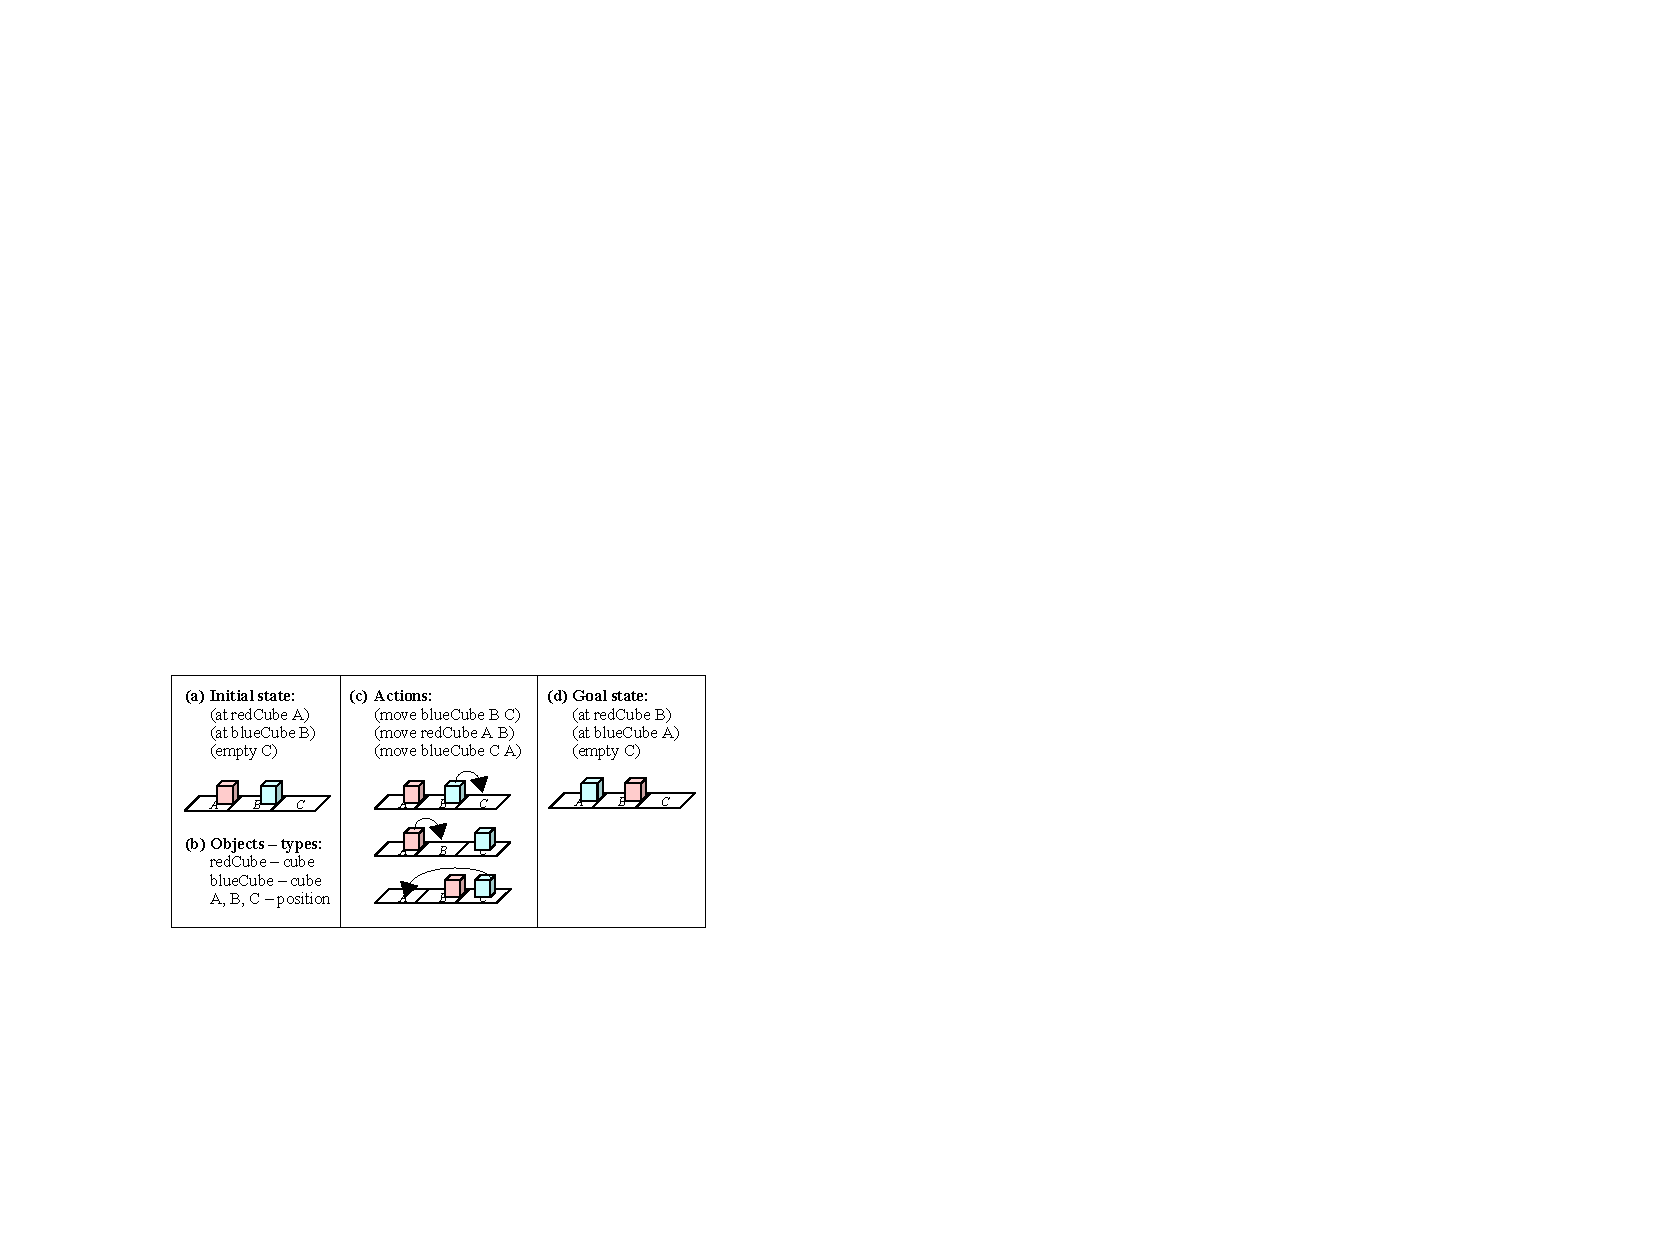
\includegraphics[width=0.7\linewidth]{figures/planning-permutation}
	\caption{Definition of a planning problem (a) properties describing the initial world state (b) object names and their types (c) instantiated actions (d) properties describing the goal state.}
	\label{fig:planning-permutation}
\end{figure}


\subsection{Results}
We did not observe any significant differences in the performance of users with or without programming experience.
9 (out of 10) participants found the symbolic representation of properties and actions easy to understand.
During the experimental test, the majority (9 or 90\%) of the participants managed to describe the complete world state using the correct syntax.
When faced with different scenarios to refine the move action model, 5 (or 50\%) of the participants struggled to formalise the \textit{stackable} condition in the symbolic language.
They provided alternative formulations related to the cube's properties (\eg `if the cube can hold the ball').
However, once the condition was defined, the majority (8 or 80\%) of the participants had little to no difficulties generalising properties, \eg defining planning operators (\fig{fig:action model}).
Due to time constraints, only 5 (or 50\%) participants were presented the planning phase.
All 5 encountered no problems when defining the action sequence to achieve the given goal.

In the questionnaire (\fig{fig:eEvaluation2}), the majority (9 or 90\%) of the participants understood the notion of states and object properties.
8 (or 80\%) correctly pointed out two properties that could not exist in the same state (\eg \texttt{(empty A)} and \texttt{(at cube A)}).
All participants gave correct explanations for preconditions and effects of action models, and provided correct examples.
9 (or 90\%) participants encountered difficulties during the experiment, 6 (or 60\%) stated problems with formalising the language, especially at the beginning of the experiment.
Half of the participants believed that they could apply this language on their own.
No participants believed that an `expert' programmer was required to learn the symbolic planning language, but 7 (or 70\%) participants believed that the minimum requirement was a `beginner' programming level, while 3 (or 30\%) believed that no programming experience was required at all.


\begin{figure}[ht]
	\centering
	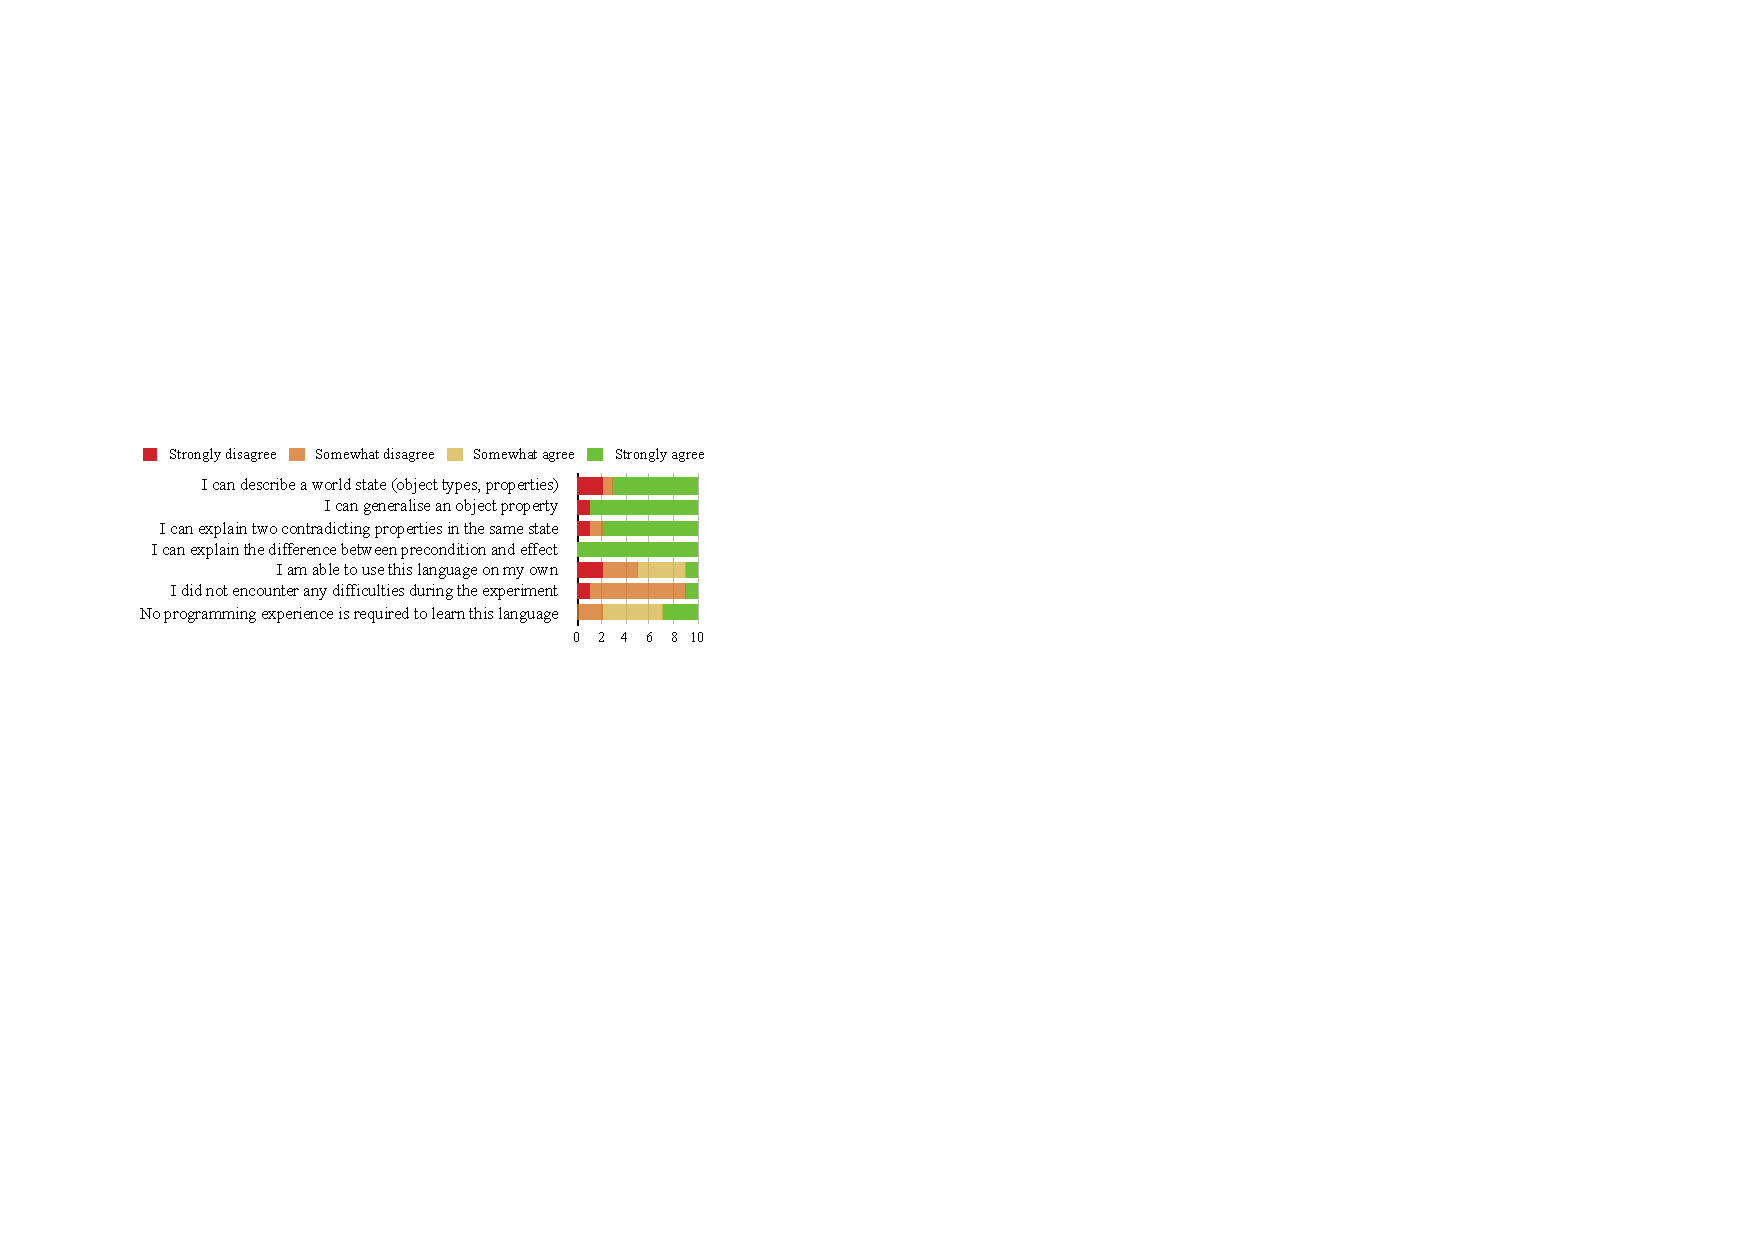
\includegraphics[width=0.85\linewidth]{figures/eEvaluation2}
	\caption{Summary of questionnaire responses: Extract of the 26 questions on the user's experience and understanding of the introduced planning language.}
	\label{fig:eEvaluation2}
\end{figure} 

\section{Experiment 2: Acceptance of the Robot Programming Framework}
\label{sec:Exp2}

In this experiment, we are addressing the following question:

\begin{enumerate}
  \item[\textbf{Q2}] Can users teach a robot action models for automated planning using the robot programming framework?
\end{enumerate}
\begin{sloppypar}
Users were presented a simulated implementation of the robot programming framework (\chapt{chap:Contribution}), and had to teach action models by kinesthetic manipulating a Baxter robot (\fig{fig:Baxter}). 
Users were instructed to demonstrate an atomic action and to assign preconditions and effects.
The goal was to assess the framework's usability and user's difficulties encountered when teaching action models.
At the end, participants were given a questionnaire related to their experience, their perceived understanding of the presented planning concepts and the usability of the framework.
The experimental protocol, questionnaire and additional material used can be found in Appendix \ref{app:exp2}.
In the following sections we briefly outline the experimental setup, measurements and results of the experiment.
%We then provide details on the partial implementation of the system used with the Wizard-of-Oz technique (\sect{ssec:WoZ}).
\end{sloppypar}

\subsection{Experimental Setup \& Participants}
We recruited 11 participants (7 male, 4 female), who were students and staff members at the Universit\'{e} Grenoble Alpes. 
6 participants reported programming experience with office productivity software (`beginner'), 2 had previously taken a programming course before (`advanced'), and 3 were pursuing studies in Computer Science (`expert').
%4 participants had previously heard of Automated Planning, but only 3 attended a related course.
The experiments were conducted using a Baxter robot (\fig{fig:Baxter}), mounted with a partial implementation of the framework.
The implemented functionalities included:
\begin{itemize}
	\item `learn new action': record the action demonstration
	\item `find a coloured object': apply the recorded action to an object of the specified colour
	\item `execute an action sequence': execute multiple actions
\end{itemize}

We used the Wizard-of-Oz technique to simulate the remaining functionalities (\eg `learn action preconditions and effects', `generate solution using a planner').
%Further details to the partial implementation are discussed in Section \ref{ssec:WoZ}.
Participants operated on a table with 2 positions D (for departure) and A (for arrival), 2 cubes (blue and red), that represented parts on an assembly line (\fig{fig:Baxter}). 
Each participant was allocated 1 hour, but the average duration was 29.5 minutes. 
The experiments were recorded, while the participant interacted with the robot. 


%The complete experimental protocol is shown in \fig{fig:Experimental protocol}. 
\subsection{Experimental Design \& Measurements}
The experiment scenario was set in a simulated assembly line, where objects of the same shape, but different colour arrived consecutively at the departure position D.
Users were told that objects were too heavy for human operators to move, hence needed to be handled by robots.
Also, due to the type of object, they should not be stacked.
Users had to teach Baxter the action for moving an object from D to arrival position A, for another maintenance task to be performed.
Throughout the experiment, users were faced with two different scenarios, where Baxter had to apply the learned move action. 
We evaluated the user's capability to refine action models and their associated conditions, when faced with different situations, and wanted to assess the framework's overall usability.

\begin{figure}[h]
	\centering
	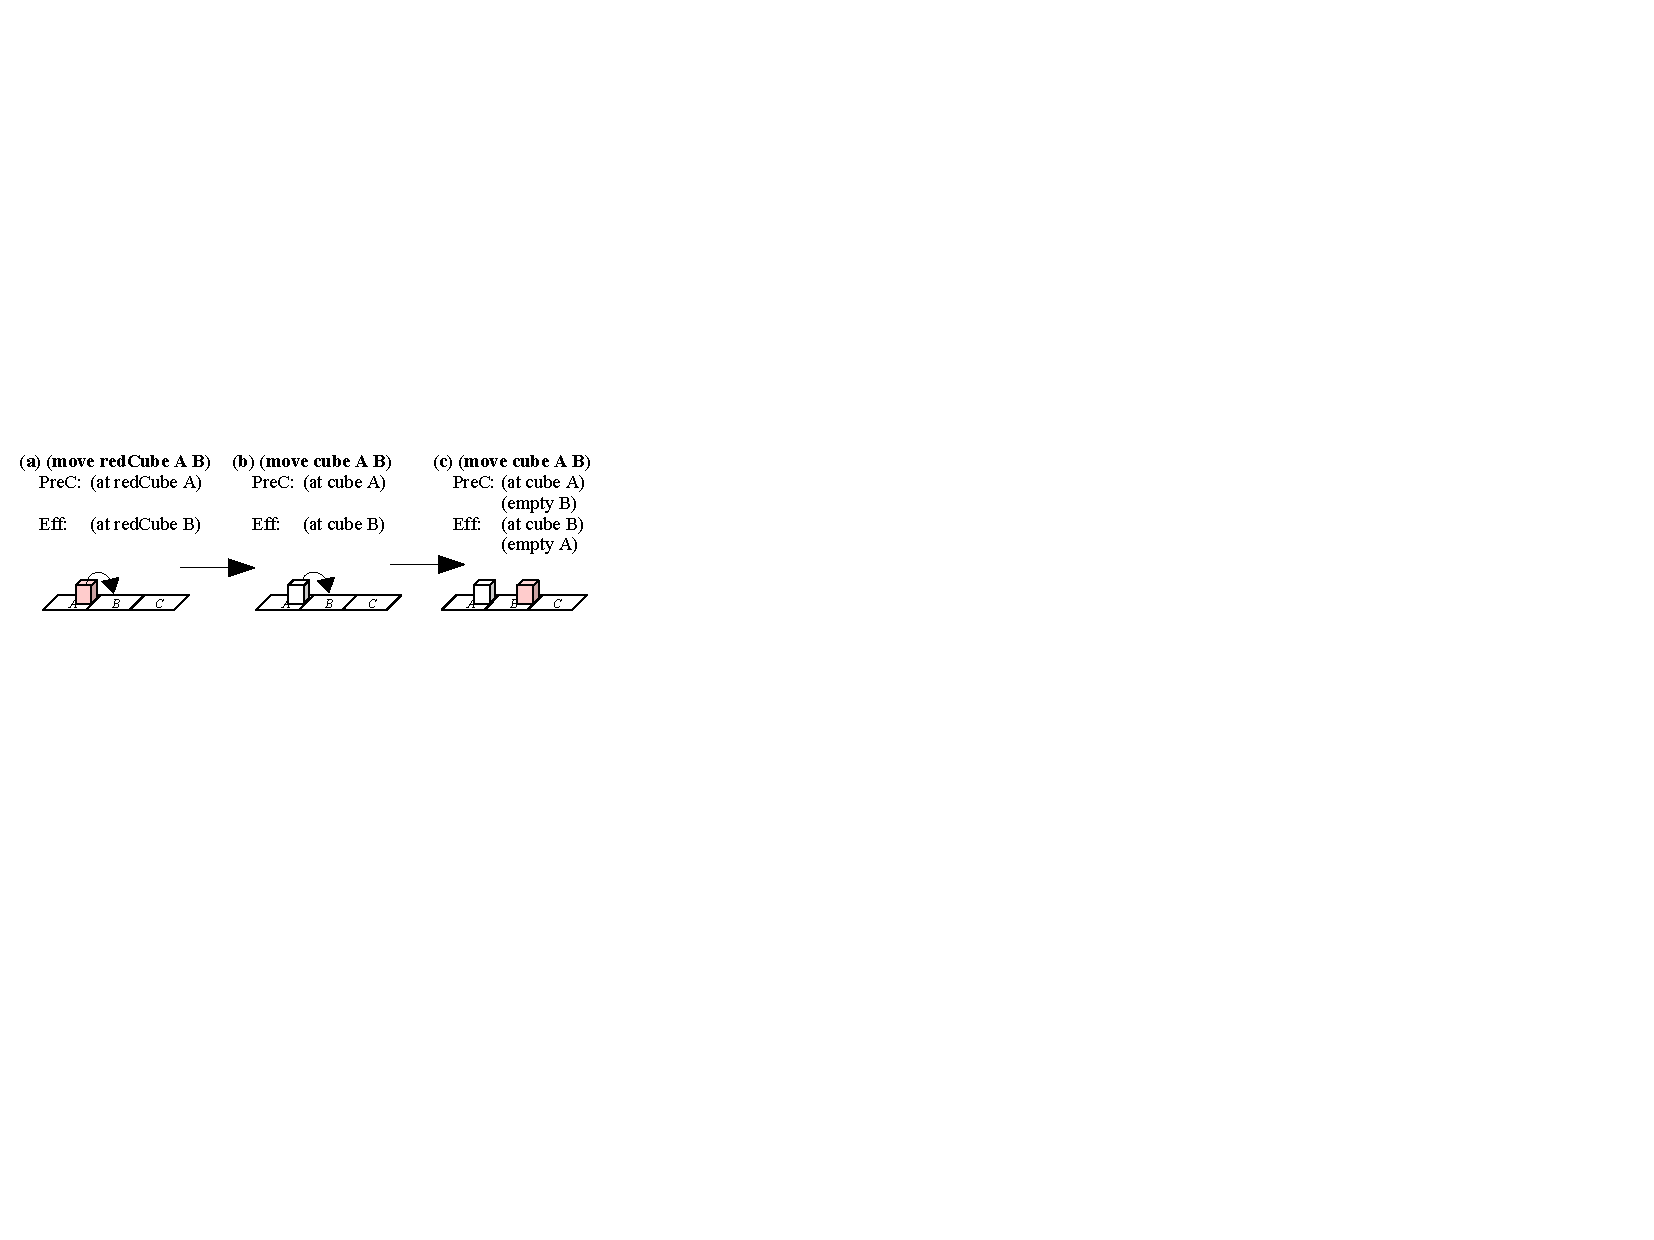
\includegraphics[width=0.8\linewidth]{figures/scenarios-exp2}
	\caption{Continuous refinement of the move action model: (a) initial action model learned by demonstration, (b) action model for all cubes of any colour, (c) action model with an additional condition, if the target position is occupied and cubes can not be stacked.}
	\label{fig:scenarios-exp2}
\end{figure} 

The experiment consisted of the following phases:
\begin{itemize}
  %\item{Introduction: After a short introduction to the Baxter robot \cite{Baxter}, users were told that they needed to use a planning language (STRIPS) to explain Baxter the state of the world and the semantic meaning of the actions.}
  \item{\textbf{Training:} Users were shown how to manipulate Baxter's arm, and given time to familiarise themselves with the kinesthetic manipulation. 
  	For this experiment we only used the robot's suction gripper to manipulate objects.}
  \item{\textbf{Experimental test:} Users were instructed to teach Baxter a move action of a red cube. 
  	Then, they were presented the action model, with preconditions and effects, that Baxter learned from the demonstration (\fig{fig:scenarios-exp2}a). 
  	In the following, users were faced with two different scenarios to refine the conditions of the action model. 
  	Starting with the initial action model for a red cube, users modified the conditions, so that it was applicable to all cubes of any colour (\fig{fig:scenarios-exp2}b), and when the target position was occupied (\fig{fig:scenarios-exp2}c). 
  	At each step, users observed how Baxter executed the learned action in the new scenario. 
  	When Baxter failed to execute the action, users had to refine the conditions of the action model.}
  \item{\textbf{Planning:} Users were presented a new scenario, where Baxter was instructed to achieve a goal using the learned action model. 
  	The new goal was to switch the positions of two cubes on the table (\fig{fig:planning-permutation}). 
  	Users first asked if they believed Baxter was able to solve this task and then shown how the taught action was reused with an automated planner.
  	Finally, Baxter executed the action sequence to complete the task.}
  \item{\textbf{Questionnaire:} Users were given a questionnaire containing 18 questions related to their experience (\eg `I did not encounter any difficulties during the experiment') and their perceived understanding of the presented concepts (\eg `I can explain how Baxter represented the preconditions of a new action'), and the usability of the framework (\eg `No programming experience is required to teach Baxter a new task').
  Participants had to give a rating on a scale ranging from `Strongly agree', `Somewhat agree', `Somewhat disagree', and `Strongly disagree'.
  The complete questionnaire can be found in Appendix \ref{app:exp2}.}
   \item{ \textbf{Debriefing:} Throughout the experiment, users were asked about their expectations on Baxter's behaviour before applying the learned action model to a new scenario. 
   	Users were asked open-ended questions (\eg ``What will Baxter do when applying the learned action model?"), so that their responses were unbiased. 
   	When they encountered failure scenarios (\eg when Baxter stacked two cubes), they were asked to reason about Baxter's behaviour and proposed modifications to the taught action model.} 
\end{itemize}

\subsection{Results}
During the experiments we observed how users learned and used the presented programming process and planning concepts.
When asked for improvements of the initial action model (\fig{fig:scenarios-exp2}a) no users pointed out missing conditions before being faced with the new scenario (\fig{fig:scenarios-exp2}c).
Even users who were `experts' and who have heard of automated planning before, did not propose a complete action model from the start. 
However, when faced with the relevant failure scenarios all users detected the missing conditions easily.
In the final phase, 8 (or 73\%) users with no experience in automated planning did not expect Baxter to solve the permutation problem, and agreed unanimously that it acted in an intelligent manner, when it did. 

Figure \ref{fig:eEvaluation} shows the user responses to the questionnaire.
All (11) users were satisfied with the PbD process and Baxter's abilities to learn and reproduce the demonstrated move action and no users encountered difficulties during the experiment. 
%All users understood the learned action model and managed to adopt the notions of preconditions and effects easily. 
At the end of the experiment, all users believed that they had taught Baxter a new task. 
The majority of users were confident that they could explain how Baxter learned and represented the new action model.
9 (or 82\%) understood the notion of preconditions and agreed that no programming experience was required to teach Baxter using the proposed framework.


\begin{figure}[h]
	\centering
	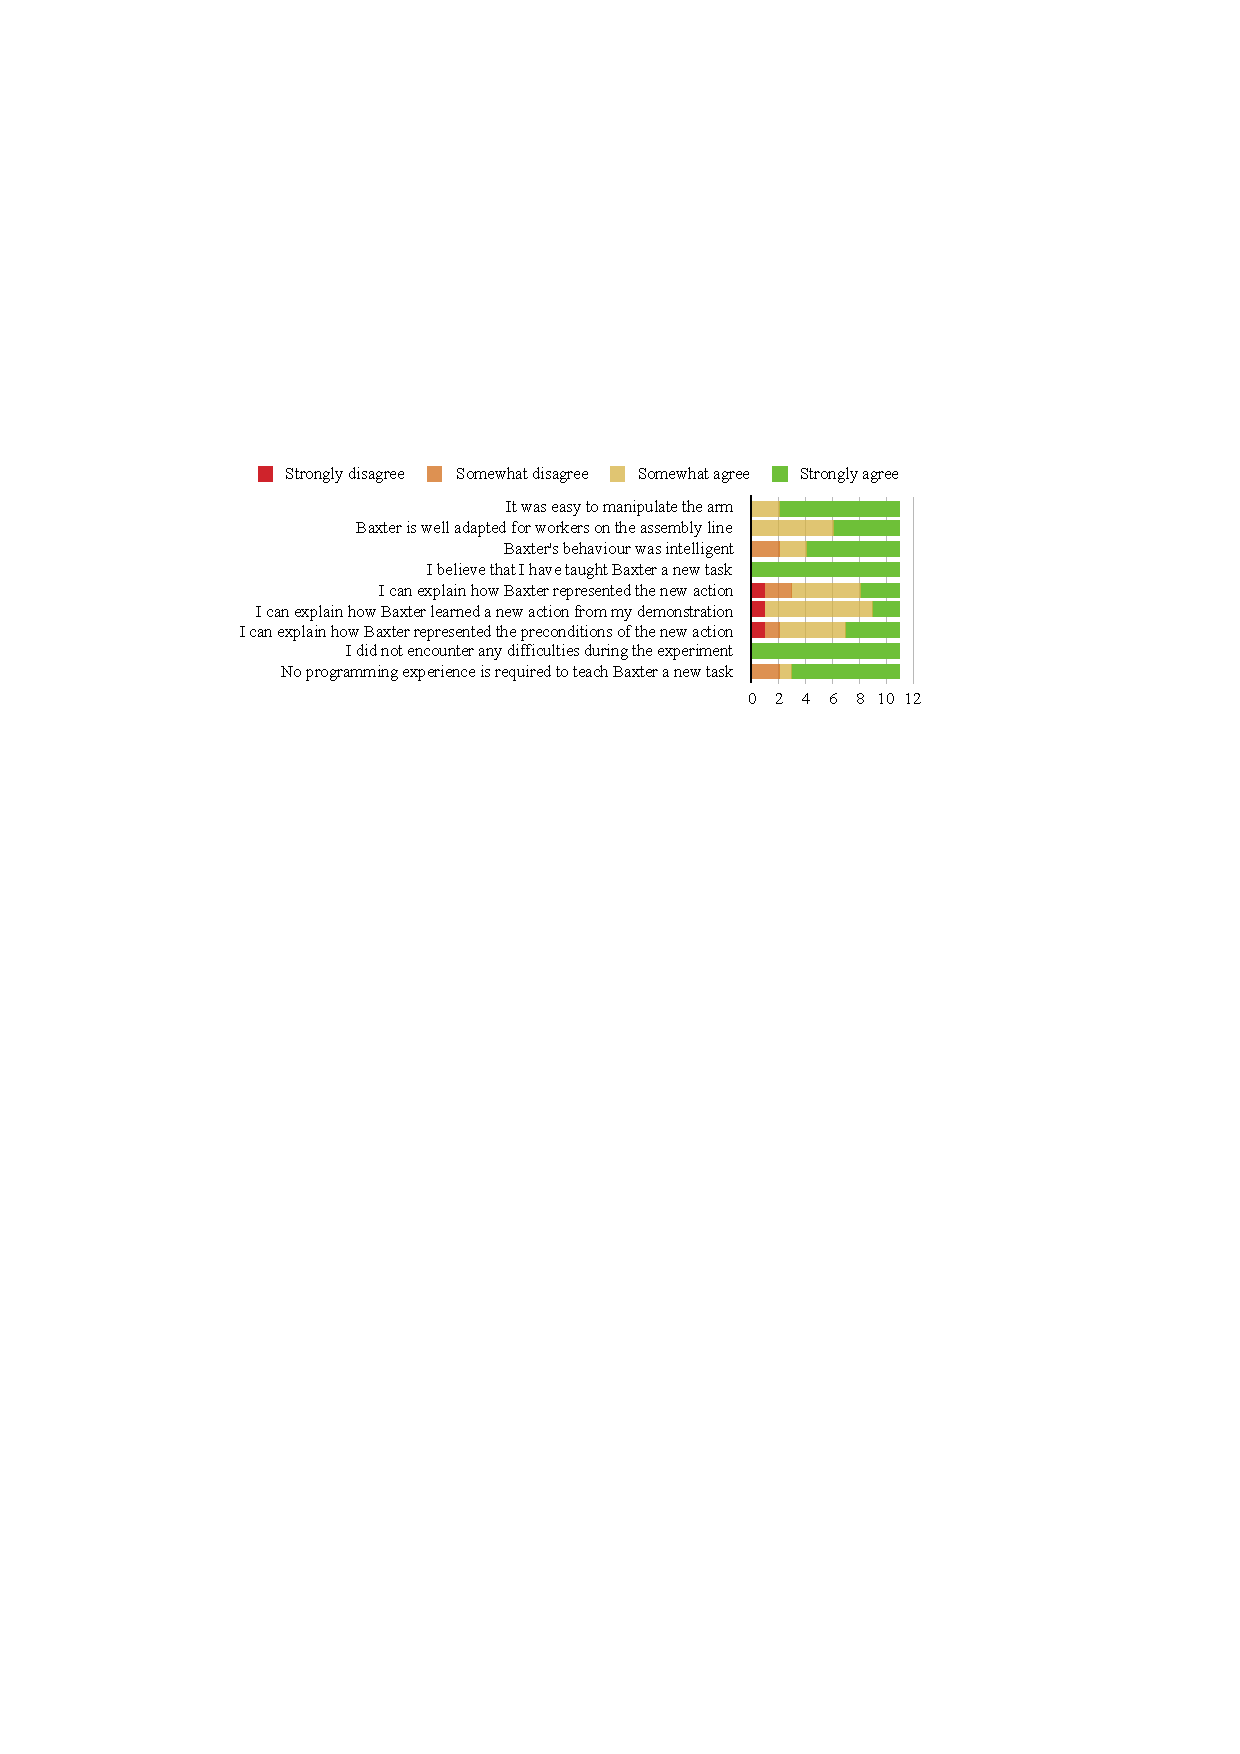
\includegraphics[width=\linewidth]{figures/eEvaluation}
	\caption{Summary of questionnaire responses: Extract of 18 questions on the user's perceived usability and understanding of the programming process after the experiment.}
	\label{fig:eEvaluation}
\end{figure}

%\section{Implementation of the Framework}
Due to the limited time-frame of this project, we aimed to evaluate the usability of our proposed framework, rather than creating a complete implementation thereof.
Hence, we focused on creating a program, which allows us to simulate a fully functional implementation of the framework, in order to conduct realistic experiments.
Our framework should allow an unexperienced user to construct action models in PDDL that can be used in a goal-oriented approach.
The actions are learned by demonstration and then used to execute complex tasks such as the permutation of objects on the table.

%We evaluated the usability of this framework in terms of experiments discussed in Chapter \ref{Evaluation}.
Consider the PbD principle overview shown in \fig{fig:Baxter-Case-Study}.
By iterating through the individual stages, we implemented our framework with the following functionalities:
\begin{itemize}
\item Search for an object,
\item Record a simple movement which represents the action,
\item Assign predicates and parameters to the learned action,
\item Create the action model in PDDL,
\item Execute a sequence of created actions defined in an external file.
\end{itemize}

  \begin{figure}[ht]
    \centering
    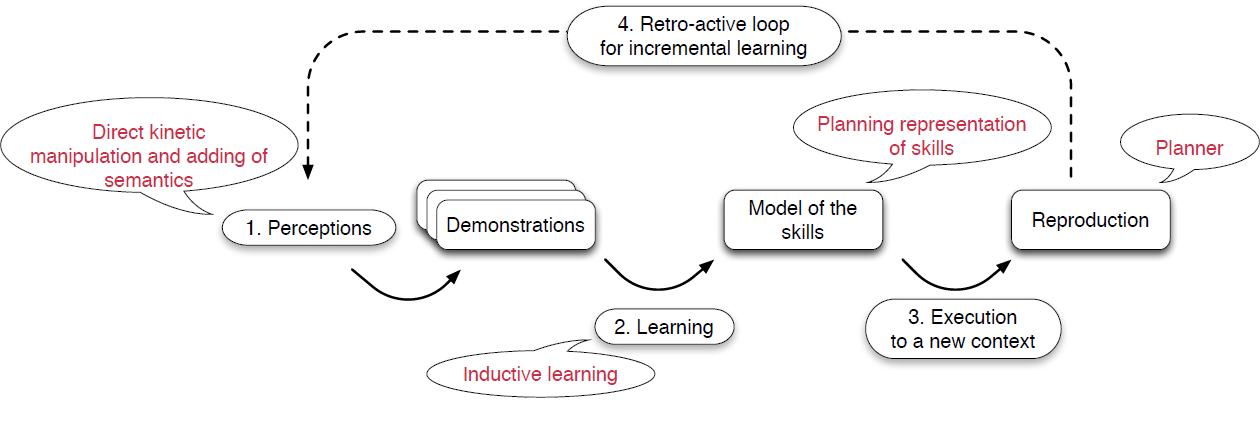
\includegraphics[scale=0.45]{figures/Baxter-Case-Study}
    \caption{PbD principle overview}
    \label{fig:Baxter-Case-Study}
  \end{figure}

%This framework allows the user to create any actions needed for the PDDL domain.
In the following sections we will discuss the implementation of each of the above mentioned functionalities in depth.

%\subsection{Intera Software}
%The industrial version of the Baxter robot currently comes with the Intera 3 software that provides a graphical user interface.
The software allows the selection of the basic tasks in order to build an action sequence.
Aimed at taking over factory operations that usually employ several people, the industrial version of Baxter can easily be taught simple tasks without the need for programming.


%%%% Step 1 %%%%
\section{Baxter Research Robot}
We implemented the framework using a Baxter Research Robot \cite{robotics2013baxter}, which is required to learn the action models needed for a pick-and-place action.
Baxter is a two-armed humanoid robot created by Rethink Robotics and introduced in 2012 \cite{robotics2013baxter}.
The SDK interfaces with Baxter via the Robot Operating System (ROS), a framework developed in 2007 by the Stanford Artificial Intelligence Laboratory, that allows the shared use of software across a wide variety of robotic platforms \cite{fernandez2015learning}.
Unlike the industrial version of the Baxter robot, which comes with the Intera 3 software that provides a graphical user interface, the research robot arrives without any such functionalities.

To date, there are many research laboratories that have started developing algorithms using the Baxter Research Robot.
Current implementations for task execution with the Baxter research robot are specifically designed to fulfill a certain task (e.g.
pick up golf balls and place them in a basket \cite{BaxterGolf}, play the game Connect 4 by picking up chips from a specified location \cite{Connect4}).
After the Ebola outbreak in West Africa in 2014, the Baxter Research Robot has been utilised to reduce the risk of contamination \cite{Ebola}.

%However, the educational level of robotics students to provide solutions for workers is far behind the potential for robots.

\section{The User Interface}
Our user interface was built upon the existing ROS package called \textsc{Baxter Tasker} created by Generation Robots \cite{BaxterTasker}.
\textsc{Baxter Tasker} is intended for the Baxter Research Robot and provides a user interface on both the computer and the robot.
The user interface was initially designed to allow users to set up a simple pick and place behaviour and provides a general overview of Baxter's capabilities.
The Python classes combine the use of sensor data and existing Baxter interface classes.
 \fig{fig:interface} shows the added functionalities.
In our implementation, we did not focus on the interface layout, hence did not modify the existing one.

  \begin{figure}[h]
    \centering
    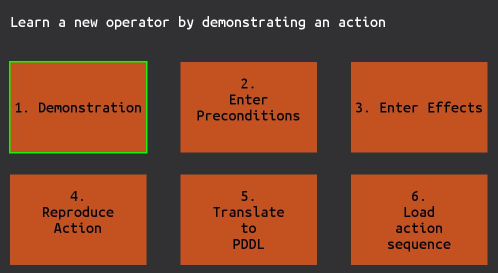
\includegraphics[scale=0.5]{figures/interface}
    \caption{Implemented Baxter interface for Programming by Demonstration}
    \label{fig:interface}
  \end{figure}


%The package includes the following functions which were particularly useful for this project:
%\begin{itemize}
%\item Conversion of pixel coordinate to limb x-y-position
%\item
%\end{itemize}



\section{Perceptions}
During the demonstration, our framework makes use of the sensors provided by the Baxter Research Robot.

As Baxter was designed for easy arm manipulation, we use teleoperation (\sect{subsec:Gathering demonstrations}) for demonstrations.
This is the most accurate way to transfer the teacher's intention to Baxter and when performing the task as the teacher handles Baxter's limb directly when demonstrating the task.
We initially considered the use of the electric gripper, but realised that it was more appropriate for precision tasks, as the gripper only allows a limited grasping area.
Suction grippers are more commonly used in manufacturing environments for the manipulation of objects with arbitrary size.
Thus, in our implementation we only use Baxter's arm with a suction gripper.
It is assumed that the searched objects have a flat surface for the vacuum gripper to grasp.

Baxter is equipped with a camera on the screen and one on each end effector.
The head camera is not very flexible, as the screen does not tilt enough.
For state observation and object localisation, we decided to only use the camera on Baxter's end effector, that is used for the manipulation task.

\subsection{Knowledge representation} 
There has been little research addressing the sharing and reuse of knowledge.
OpenCyc \cite{lenat1990cyc}
OpenRobots Ontology (ORO) \cite{lemaignan2010oro} creates an abstract representation for high-level knowledge that can be shared among multiple platforms.
In \cite{lemaignan2017artificial} it is loaded as a priori knowledge and used as an active knowledge base to manage symbolic facts and beliefs produced and shared by cognitive modules such as language processing, task planning, or geometric reasoning modules.
The authors gather knowledge from three sources: a priori knowledge, knowledge acquired at run-time from perception, and symbolic statements from inferences produced by the reasoner.
SPAtial Reasoning\&Knowledge (SPARK) \cite{sisbot2011situation} is a geometric and temporal reasoning module that can produce symbolic statements to describe the state of the robot environment and its evolution over time, e.g. <BOOK1 type Book, BOOK1 isOn TABLE>, \\
find(BOOK2 isAt ?location) \\
find(?obj type Book, ?obj differentFrom BOOK1)\\
TAPE isVisible true \\
TAPE isReachable true\\ 
TAPE isOn TABLE\\
TAPE isIn BIN\\
ROBOT hasInHand TAPE\\
\cite{lemaignan2017artificial} use 2D fiducial markers for object recognition and have about 10 markers present during the experiment at a time.
RoboEarth \cite{waibel2011roboearth} collects, stores, and shares data independent of the robot hardware to allow reuse of data for robotic platforms.
Other approaches include the CRAM/KnowRob architecture \cite{bibid} the knowledge base is an active hub that pro-actively queries perceptual components to acquire knowledge.

We defined a set of types and predicates for our domain model 

 
%%%% Step 2 Learning %%%%
\section{Learning}
%%%% Model of the skills %%%%
%\subsection{Create an action model}
\label{Create an action model}
Recall the action models in PDDL as part of the \texttt{PRODUCTION} domain mentioned in \sect{subsec:Planning domain description}.
In order to teach Baxter a complete pick-and-place action, we need to teach Baxter all action models (pick, move, drop) to solve the \texttt{PERMUTATION} planning problem.
It is sometimes necessary to teach the robot all basic component actions separately, as they all have varying preconditions and effects.
The user should be able to create each of these action models by demonstrating the action and letting Baxter derive the associated conditions.
 %This includes opening and closing the gripper, as well as the limb movement itself.


Thus, a simple pick-up action should be demonstrated as approaching the object, closing the gripper and lifting the object vertically.
An example of the observed action model of a \texttt{pick} action with the Baxter's right limb, grasping a red-coloured object at a starting position $(0,0)$ is the following:

\begin{verbatim}
   (:action pick
       :parameters (red - product 0-0 - location right - gripper)
       :precondition  (and  (at red 0-0) (at-gripper right 0-0) 
              (free right) not(empty 0-0))
       :effect (and (carry red right)
   (empty 0-0)
   (not (at red 0-0)) 
   (not (free right))))
\end{verbatim}
In order to execute the action, the robot observed that the red-coloured product was at location 0-0 and that the right gripper was free.
The effect of the \texttt{pick} action was that the right gripper was carrying the red product and that it was no longer occupying position 0-0.
Instead of replicating the demonstrated movement, the robot extracts the relevant characteristics of the gesture that need to be reproduced.
%To learn the action, it needs to observe the main attributes that can change and that are relevant to reproduce the action.
The world before and after each action is observed and the change is then recorded.


The above action model shows the learned \texttt{pick} action with the observed preconditions and effects, before and after the action execution.

The robot learns a generalised action model by removing the instantiated values for the variables \texttt{product}, \texttt{position} and \texttt{gripper}:

\begin{verbatim}
   (:action pick
       :parameters (?p - product ?l - location ?g - gripper)
       :precondition  (and  (at ?p ?l) (at-gripper ?g ?l) (free ?g))
       :effect (and (carry ?p ?g)
      (not (at ?p ?l)) 
      (not (free ?g))))
\end{verbatim}

\subsubsection{Implementation}
Due to the limited scope of this project, we only implemented the observed characteristics that were crucial to reproduce the action (see Table \ref{tab:PDDL implementation}).
For predicates describing the object's state, we would need to use a second camera, as the one on the end effector would have a restricted view after the grasping an object.

\begin{table}[h]
\begin{center}
\begin{tabular}{l|l}
PDDL & Implementation\\ \hline
\texttt{:action pick} & action_name: String\\
\texttt{at-gripper ?g ?l} & change_vector: Pose\\
\texttt{free ?g } & gripper_change: Bool\\
\texttt{carry ?p ?g} & holding_object: Bool
\end{tabular}
\label{tab:PDDL implementation}
\caption{Implementation of the PDDL predicates}
\end{center}
\end{table}

The \texttt{change_vector} is the trajectory calculated by taking the difference between the gripper's initial pose and goal pose.
This allows a learned movement to be reproduced from any arbitrary gripper position.
The \texttt{gripper_change} variable states whether or not the gripper status should be changed (between open and close) or whether it should be simply ignored.
The \texttt{holding_object} attribute (see Section \ref{holdingObject}) indicates whether the gripper is currently holding an object.

%\begin{table}[h]
%\begin{center}
%\begin{tabular}{l|l}
%Action name & Observed attribute changes\\ \hline
%Move horizontically & End effector's position\\
%Move vertically & End effector's position\\
%Rotate gripper pose & End effector's pose\\
%Grasp object & gripper status \\
%\end{tabular}
%\end{center}
%\label{tab:Action examples}
%\caption{Examples of possible actions to be learned}
%\end{table}

Our implementation only considers one demonstration for the learning process.
Different learning algorithms (e.g.
Bayesian, neural networks) might be required to improve the performance of the learned trajectories by taking into consideration multiple demonstrations.

Furthermore, in order to allow planning for more complex control structures in real-world domains, it is necessary to detect divergences of the planned states from actual sensed states.
The use of multiple cameras would be required to verify the actual states.
%\cite{ObjectActionComplexes} Another possibility is to learn a visual object model of an unknown object by grasping it to allow grasping different kinds of objects.

%\subsubsection{Learning preconditions and effects}
After the demonstration of the action, the user needs to verify the observed conditions associated with the action.
Due to the limited time and scope of this project, we did not implement the translation of the internal action model into PDDL.
However, the user can select the predicates to be associated with the action via the user interface.
The user interface proposes all predicates provided in the domain description and generates the PDDL code according to the user's selections.
In future work this could be automated, such that these predicates are automatically recognised by the robot from the taught action.

\section{Reproduction}
After the creation of all action models, the user should be able to reproduce a task as a combination of all actions, in order to validate its usability.
We consider the pick-and-place action of an object as a sequence consisting of four subtasks:
\begin{enumerate}
\item Reach the grasp position: align the gripper vertically with the object, i.e.
\texttt{search}
\item Grasp the object: approach the object vertically and close the gripper, i.e.
\texttt{pick}
\item Move the object: perform the learned limb movement to the goal position while holding the object, i.e.
\texttt{move}
\item Place the object on its goal position: open the gripper to release the grasped object, i.e.
\texttt{drop}
\end{enumerate}

\subsection{Reach the grasp position}\label{Object Search}
The skill of searching an object will have to be an inbuilt functionality, which can't be learned by demonstration.
Possible extensions are to learn the shape and colour of new objects to be searched.
We considered the possibility of using QR codes to identify objects, but realised that an RGB colour search was more efficient and intuitive for our experimentations.
Furthermore, we considered tracking the object on-line using the camera.
As objects in our environment are static, this would be unnecessary, so we decided against it.
Thus, the search is performed on a picture that is regularly taken by the camera after a position change.

We used OpenCV, as there already exists a library that allows simple edge detection and object recognition from pictures.

At the beginning of the search, the camera is moved to a position where the entire working area can be captured in the image.
Using the OpenCV library \cite{opencv}, we convert this image to a bit array and filter by the searched colour to track the location of an object.

Once the greatest area containing the searched colour has been identified, the grasp position is calculated by taking its center (see \fig{fig:detectObject1}).

We then convert the pixel location in the camera image to the x-y-coordinate of Baxter's end effector position and move the end effector by the position offset.
We iterate through this process by taking a picture with the updated camera position (see \fig{fig:detectObject2}) and calculate the distance to the object.
By repeatedly moving the camera towards the center of the object, we aim to align the center of the camera image with the center of the object.
The algorithm takes into account Baxter's positional accuracy of the joints ($\pm 5$ mm), hence stops when it has been sufficiently aligned.
\begin{figure}[h]
\centering
\begin{minipage}{0.5\textwidth}
  \centering
    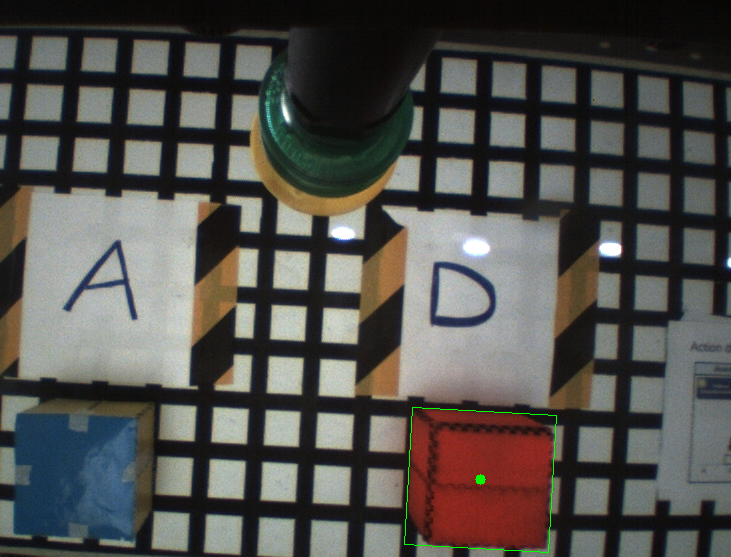
\includegraphics[scale=0.35]{figures/detectObject1}
    \caption{First iteration object detection}
    \label{fig:detectObject1}
\end{minipage}%
\begin{minipage}{.5\textwidth}
  \centering
    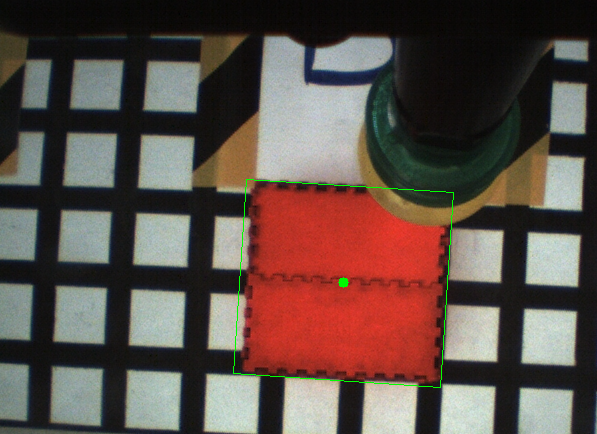
\includegraphics[scale=0.45]{figures/detectObject2}
    \caption{Second iteration object detection}
    \label{fig:detectObject2}
\end{minipage}
\end{figure}

The simplified pseudo code for the search algorithm is as follows:

\begin{verbatim}
recognise entire working area
while error rate > error tolerance
        error = distance of camera center to object center
        position offset = distance of object center to actual image center
        convert position offset to limb x-y-coordinates
	move arm closer to object by converted offset
move arm by camera to gripper offset
\end{verbatim}
Aligning the end effector with the object center is particularly important, as the suction gripper can only grasp the object, if gripper is entirely placed on the homogenous surface.
Grasping the object at the edge can lead to the object being dropped during the execution of the limb movement.

\subsection{Grasp the object}
After the gripper has been vertically aligned with the object, the learned \texttt{pick} action should grasp the object.
In the general case, the \texttt{pick} action should be learned by demonstration, as different robots have different grippers.
However, for the purposes of conducting experiments to evaluate our framework, we implemented an approach function, which replaces the \texttt{pick} action.
Depending on the assumptions made upon the objects in the domain and considering Baxter's sensor limitations, we considered several implementations of this function:
\begin{itemize}
\item Fixed height approach: All objects in this domain have the same height, hence the distance between end effector and object is constant.
The vertical approach can be fixed to a constant movement in the implementation code.
\item Flexible object height: Objects have different sizes, hence the distance to the object is not constant.
The vertical approach uses the end effector's range sensor and approaches the object until it detects the object in a close distance.
\end{itemize}
We implemented an approach function to deal with varying object heights using Baxter's infrared range sensor.
However, range sensors can return unreliable values, depending on the surface of the object (matte or glossy).
Moreover, the placement of the end effector at the edge of an object -- e.g.
for objects with small surfaces -- can skew the returned values.
One possibility to address this problem is to verify that the end effector is still approaching the object and not remaining static.


Depending on the robot's capabilities, there are many other potential implementations for this function.
For example, the user interface could provide an option to specify the object's height, or if the range sensor is reliable enough, then the object distance could be observed as part of the learning process.
For our experiments, we assumed that all objects in the domain were of the same height and, therefore, used the fixed height approach.


\subsection{Move the object}\label{holdingObject}
The move action is learned by demonstration and executed using the learned action model described in Section \ref{Create an action model}.
However, during the action execution, we need to make sure that the gripper is grasping the object.
Previously mentioned limitations (e.g.
due to the implementation of the approach function) or other unforseen problems can influence a successful grasp of the object.
As we experienced during our implementation tests, the surface of the object has to be entirely homogeneous, otherwise the object will be dropped after it has been lifted.
Thus, it is crucial to keep track of the gripper, i.e.
whether it is still holding the object during the execution of the subsequent actions.
This can be associated with the \texttt{carry ?p - product ?g gripper} predicate.
In this respect, we created a function \texttt{holding_object}, which returns the correct state, depending on the infrared range sensor (gripper is within a certain distance to the object) and the gripper status (suction is activated).

%%%% Step 3 %%%%
\section{Execution to a new context}
Combining all four subtasks allows us to reproduce the learned action in a new context.
The user interface offers the possibility to reproduce the learned actions in any arbitrary order.
This allows the user to verify whether the learned actions correspond to the demonstrated behaviour or not, and how the actions perform in different contexts.

\subsection{Goal-oriented programming}
Recall that our final objective is to teach Baxter a goal-oriented behaviour using automated planning techniques.
The user has completed the domain description with the created action models.
Given a domain, an initial state and a goal state, the automated planner will generate an action sequence that allows an efficient traversal from the initial state to the goal state.

To recognise the initial state of the world, we implemented a simple object localisation function using \texttt{object search} (see Section \ref{Object Search}), which saves the positions of the objects on the table.
Connecting the Baxter interface with an automated planner is a separate task, which we did not manage to implement in the restricted time of this project.
However, in our final implementation, Baxter can execute any sequence of actions listed in an external text document.
This allowed us to simulate an execution of a plan generated by an automated planner.

Note that in our implementation, we rely on a general assumption on the objects included in the domain.
The object search function assumes that all objects have a monotonous colour and a flat and homogeneous surface that guarantee a successful execution of the implemented \texttt{approach} and \texttt{holding_object} functions.

%In Section \ref{Conclusion} we will discuss possible extensions and respective implementations which allow the manipulation of other object types.


%Since we assume that there is only one gripper, the \textbf{gripperFree()} attribute does not take any arguments.
%For this simplified planning domain, we restrict the attributes to allow only objects of type block.
%
%\begin{table}[h]
%\begin{center}
%\begin{tabular}{l|l|l|l}
%Action & Precondition & Effect\\ \hline
%move\_block(X,Y) & block\_at\_position(X,Y) and clear(Z) & block\_at\_position(X,Z) and $X \neq Z$ \\
%grasp(X) & gripper\_free() & not(gripper\_free())\\
%\end{tabular}
%\end{center}
%\label{tab:actionmodels}
%\caption{Action models }
%\end{table}%

%%%% Step 4 %%%%
\section{Retro-active loop for incremental learning}
After the new action has been created and tested, it is likely that the user needs to modify or improve them.
The execution to a new context provides the user with the possibility to test the selected predicates associated with the action.
The user can take advantage of the robot's incremental learning process.
This means the repeated use of action demonstrations by the teacher and the refinement of the action model.
Multiple demonstrations can be used to extract conditions that are commonly observed and learned trajectories can be refined by using statistical modeling techniques \cite{ude1993trajectory}.
Hidden Markov Models (HMMs) can be used to encode temporal and spatial variations or to reproduce various motions \cite{tso1996hidden}.
%\section{Generate and save the PDDL code for the learned action}


\section{Discussion and Limitations}
In both experiments, we did not observe a significant difference in the performance between users with different programming experience. 
The majority of users had issues formulating the logical representations of object properties used in action models. In the first experiments, users had difficulties formulating a single condition (e.g. \texttt{(stackable ball cube)}), but stated equivalent conditions (\textit{`only place the ball, if it is stackable on the cube'}).
Similarly, in the second experiment, users formulated the missing precondition (\textit{`position B is empty'}) with other equivalent conditions (\textit{`Do not place the object on position B, if it is occupied'}). This means, that users should be provided with a predefined set of conditions that can be added to the action model.

Some users made wide assumptions about the robot's capabilities. In the second experiments, when both arrival and departure positions were occupied (Fig. \ref{fig:scenarios-exp2}c), less half of the users (5) expected Baxter to consider the occupied position, even though the condition was not mentioned in its action model.
This is a common problem in PbD solutions as there is a difference in the perception of the robot's intelligence perceived by its teacher (\cite{suay2012practical}) and can be addressed by reproducing the learned task in a new context and verifying the robot's knowledge base, as we did throughout the experiment.

With these two qualitative experiments, we showed that the automated planning language could easily be adopted by users without any programming background. Moreover, the action model representation, in terms of preconditions and effects, seems to be intuitive for non-expert users. 
However, these initial experiments only provide us with an idea of how the users might perceive the proposed framework. We intentionally limited the set of concepts that are necessary to use the framework to the bare minimum. Further experiments should test scalability and address more complicated actions involving separate control groups (experts vs non-experts) in less structured scenarios. 

